% ---------------------------------------------------------------------
% Basic configuration and packages
% ---------------------------------------------------------------------
% Package for discovering wrong and outdated usage of LaTeX.
% More information to be found in l2tabu English version.
\RequirePackage[l2tabu, orthodox]{nag}
% Class of LaTeX document: [size of paper, size of font]{document class}
\documentclass[a4paper,11pt]{article}



% ---------------------------------------
% Packages not tied to particular normal language
% ---------------------------------------
% This package should improved spaces in the text.
\usepackage{microtype}
% Add few important symbols, like text Celcius degree
\usepackage{textcomp}



% ---------------------------------------
% Polonization of LaTeX document
% ---------------------------------------
% Basic polonization of the text
\usepackage[MeX]{polski}
% Switching on UTF-8 encoding
\usepackage[utf8]{inputenc}
% Adding font Latin Modern
\usepackage{lmodern}
% Package is need for fonts Latin Modern
\usepackage[T1]{fontenc}



% ---------------------------------------
% Setting margins
% ---------------------------------------
\usepackage[a4paper, total={14cm, 25cm}]{geometry}



% ---------------------------------------
% Setting vertical spaces in the text
% ---------------------------------------
% Setting space between lines
\renewcommand{\baselinestretch}{1.1}

% Setting space between lines in tables
\renewcommand{\arraystretch}{1.4}







% ---------------------------------------
% Packages for scientific papers
% ---------------------------------------
% % Switching off \lll symbol, that I guess is representing letter ``Ł''.
% % It collide with `amsmath' package's command with the same name
% \let\lll\undefined
% % Basic package from American Mathematical Society (AMS)
\usepackage[intlimits]{amsmath}
% % Equations are numbered separately in every section.
% \numberwithin{equation}{section}

% Package with support of physical units
\usepackage{siunitx}





% ---------------------------------------
% Packages for working with graphics
% ---------------------------------------
\usepackage{graphicx}





% ---------------------------------------
% BibLaTeX
% ---------------------------------------
% Package biblatex, with biber as its backend, allow us to handle
% bibliography entries that use Unicode symbols outside ASCII.
\usepackage[
language=polish,
backend=biber,
style=alphabetic,
url=false,
eprint=true,
]{biblatex}

\addbibresource{SystemyOperacyjneBibliography.bib}





% ------------------------------
% Package ``hyperref''
% They advised to put it on the end of preambule
% ------------------------------
% It allows you to use hyperlinks in the text
\usepackage{hyperref}










% ------------------------------------------------------------------------------------
% Defining title and author of the text
\title{Systemy operacyjne \\
  {\Large Pomocnicze zdjęcia i~rysunki}}

% \date{}
% ------------------------------------------------------------------------------------










% ####################################################################
\begin{document}
% ####################################################################





% ######################################
% Title of the text
\maketitle
% ######################################





% ######################################
\section{Ludzie dzięki którym powstał system operacyjny
  GNU/Linux}

\label{sec:Ludzie-dzieki-ktorym-ETC}
% ######################################



% % ###################
% \begin{figure}

%   \centering


%   \includegraphics[scale=0.15]
%   {./Pictures/OS-heroes-Pictures/Ken-Thompson.jpg}

%   \caption{Ken Thompson (ur.~1943), główny twórca systemu Unix.}

%   \label{fig:Ken-Thompson}

% \end{figure}
% % ###################





% % ###################
% \begin{figure}

%   \centering


%   \includegraphics[scale=0.3]
%   {./Pictures/OS-heroes-Pictures/Dennis-Ritchie.jpeg}

%   \caption{Dennis Ritchie (1941--2011), współtwórca Unixa, na~potrzeby
%     napisania nowej wersji tego systemu stworzył język~C. Za~datę powstania
%     tego języka możemy uważać rok~1972~r.}

%   \label{fig:Dennis-Ritchie}

% \end{figure}
% % ###################





% % ###################
% \begin{figure}

%   \centering


%   \includegraphics[scale=0.15]
%   {./Pictures/OS-heroes-Pictures/Richard-Stallman.jpeg}

%   \caption{Richard Matthew Stallman (ur.~1953). W~1983 rozpoczął działanie
%     GNU Project.}

%   \label{fig:Richard-M-Stallman}

% \end{figure}
% % ###################





% % ###################
% \begin{figure}

%   \centering


%   \includegraphics[scale=0.8]
%   {./Pictures/OS-heroes-Pictures/Andrew-S-Tanenbaum.jpeg}

%   \caption{Andrew S.~Tanenbaum (ur.~1944). W~roku 1988 stworzył system
%     \textsc{minix} (ang.~\textit{mini-Unix}).}

%   \label{fig:Andrew-S-Tanenbaum}

% \end{figure}
% % ###################





% % ###################
% \begin{figure}

%   \centering


%   \includegraphics[scale=0.35]
%   {./Pictures/OS-heroes-Pictures/Linus-Torvalds.jpg}

%   \caption{Linus Torvalds (ur.~1969). W~roku 1991 roku stworzył jądro
%     systemu Linux (\textit{Linus + Unix}).}

%   \label{fig:Linus-Torvalds}

% \end{figure}
% % ###################










% ######################################
\section{Powłoki}

\label{sec:Powloki}
% ######################################



% ###################
\begin{figure}

  \centering


  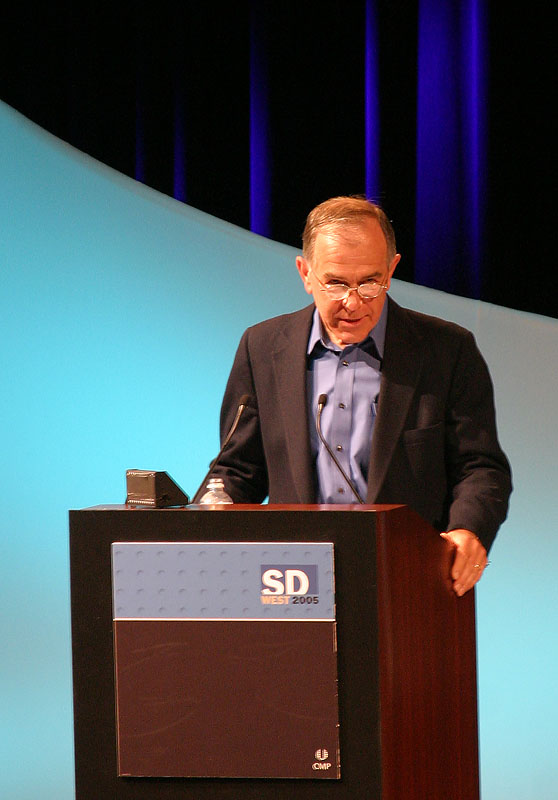
\includegraphics[scale=0.9]
  {./Pictures/OS-heroes-Pictures/Steve-Bourne.jpeg}

  \caption{Stephen Bourne (ur.~1944). W~1979~roku stworzył powłokę Bourne’a.}

  \label{fig:Stephen-Bourne}

\end{figure}
% ###################





% ###################
\begin{figure}

  \centering


  \includegraphics[scale=0.08]
  {./Pictures/OS-heroes-Pictures/Brian-J-Fox.png}

  \caption{Brian J.~Fox (ur.~1964). W~1989~r. stworzył powłokę
    \textsc{bash} (ang. \textit{Bourne-again shell}).}

  \label{fig:Brain-J-Fox}

\end{figure}
% ###################










% ######################################
\section{Maszyny}

\label{sec:Maszyny}
% ######################################



% ###################
\begin{figure}

  \centering


  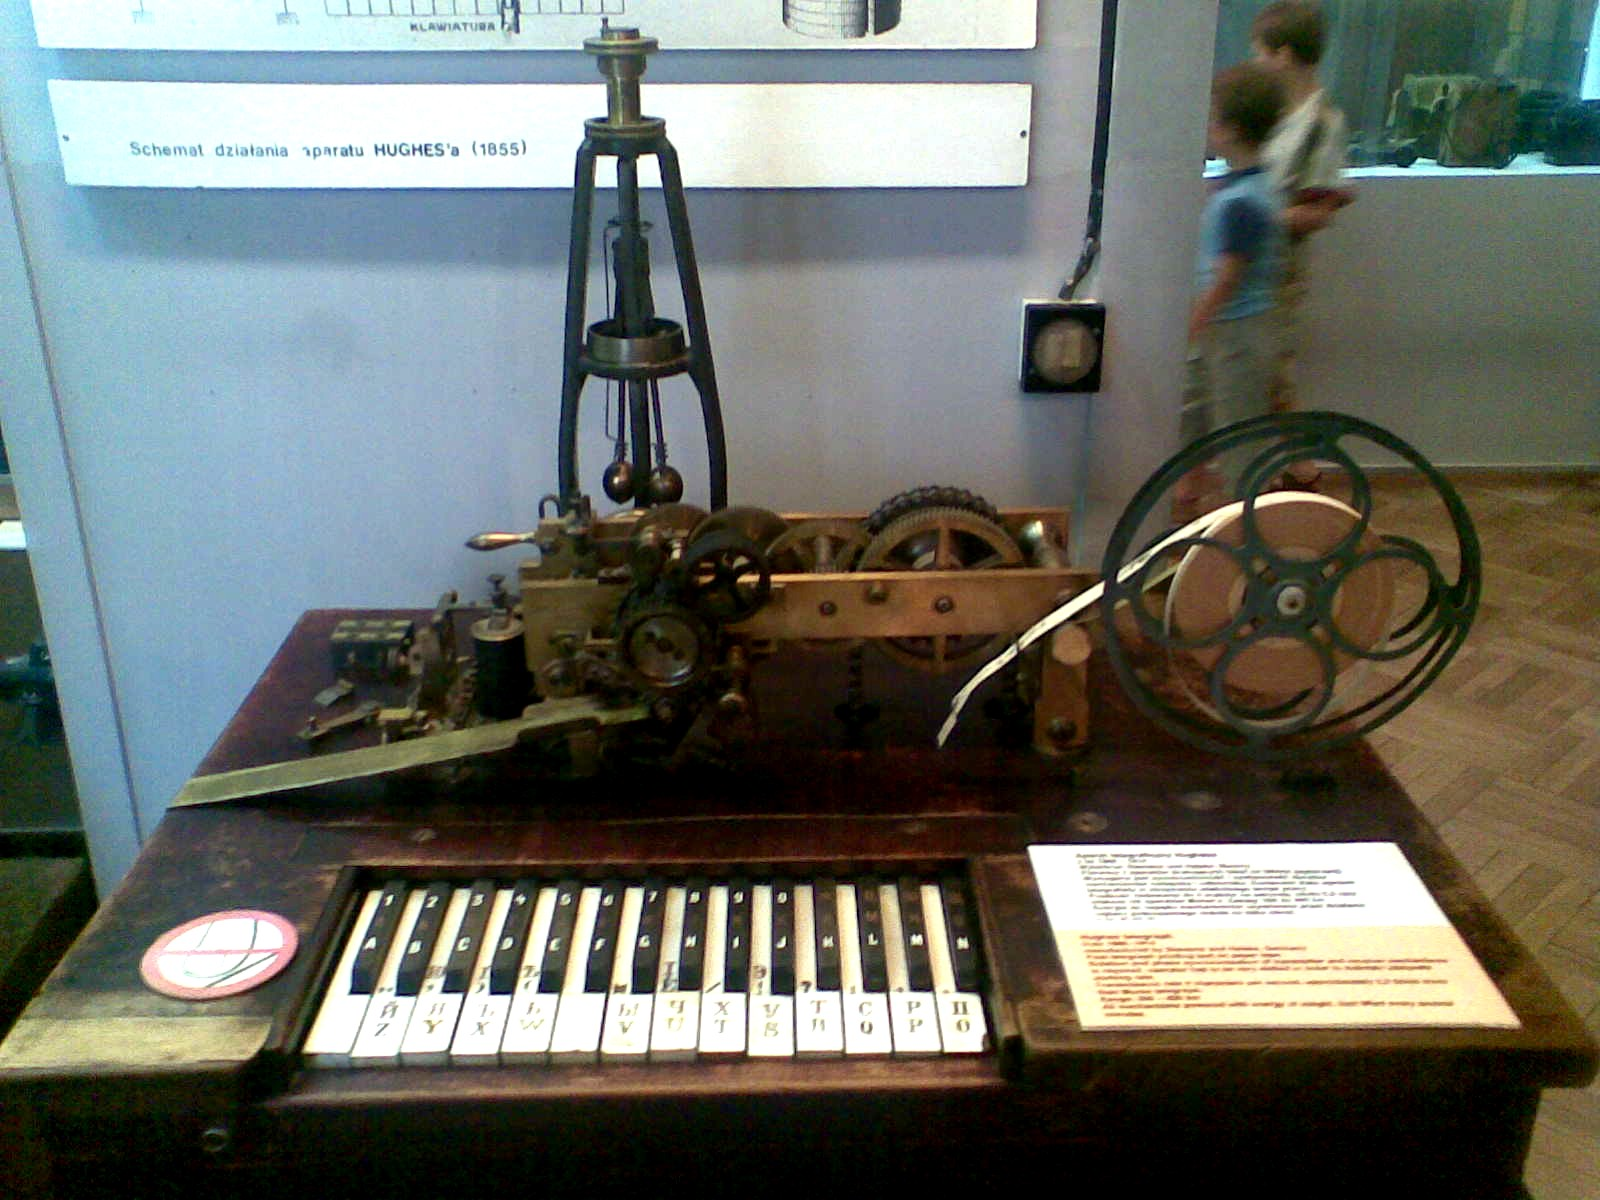
\includegraphics[scale=0.9]
  {./Pictures/Machines-Pictures/Hughes-telegraph.jpeg}

  \caption{Dalekopis zaprojektowany przez Davida Edwarda Hughesa
    (1830-1900), wyprodukowany około 1855 roku.}

  \label{fig:Dalekopis-Hughesa}

\end{figure}
% ###################





% ###################
\begin{figure}

  \centering


  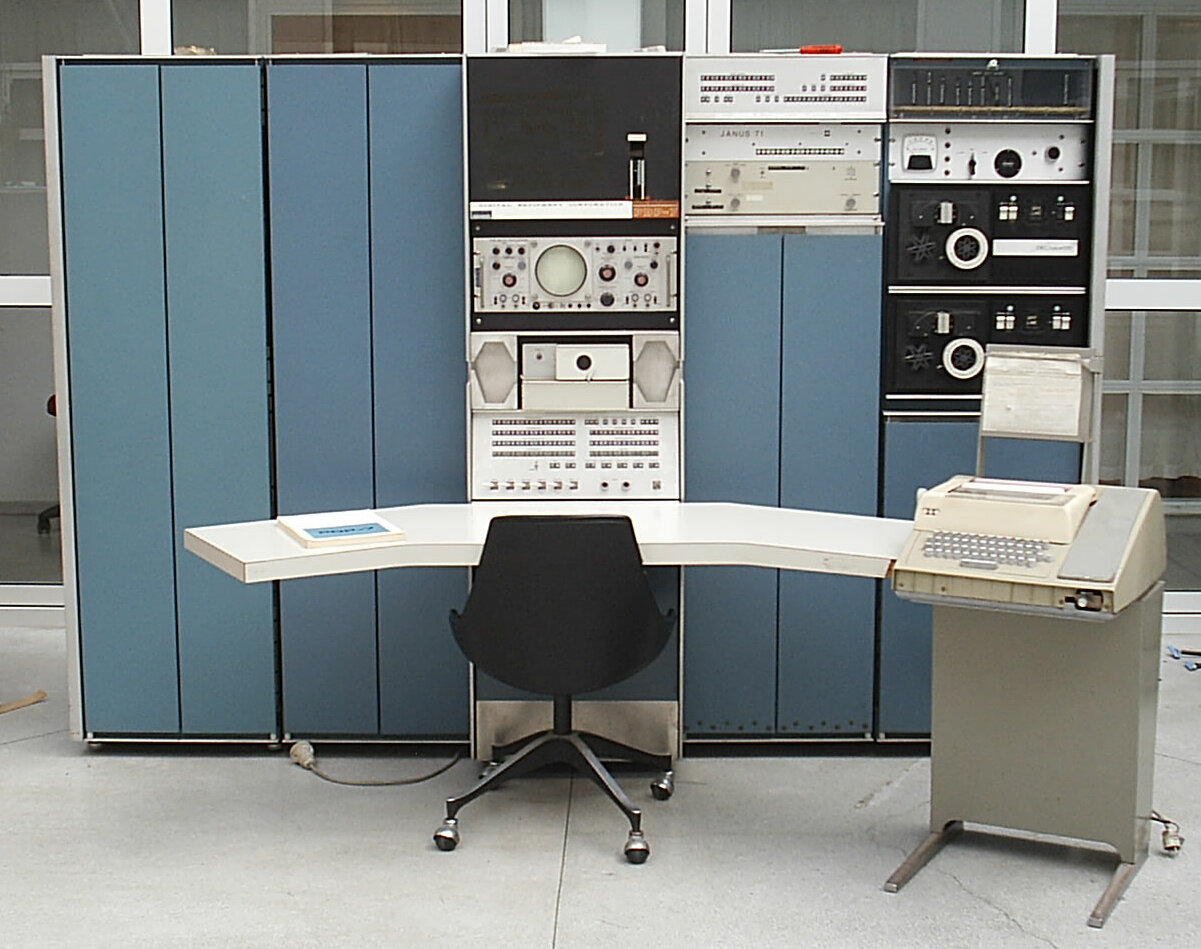
\includegraphics[scale=0.3]
  {./Pictures/Machines-Pictures/PDP-7-with-teletype.jpeg}

  \caption{Komputer PDP-7 z~dalekopisem.}

  \label{fig:PDP-7-z-dalekopisem}

\end{figure}
% ###################





% ###################
\begin{figure}

  \centering


  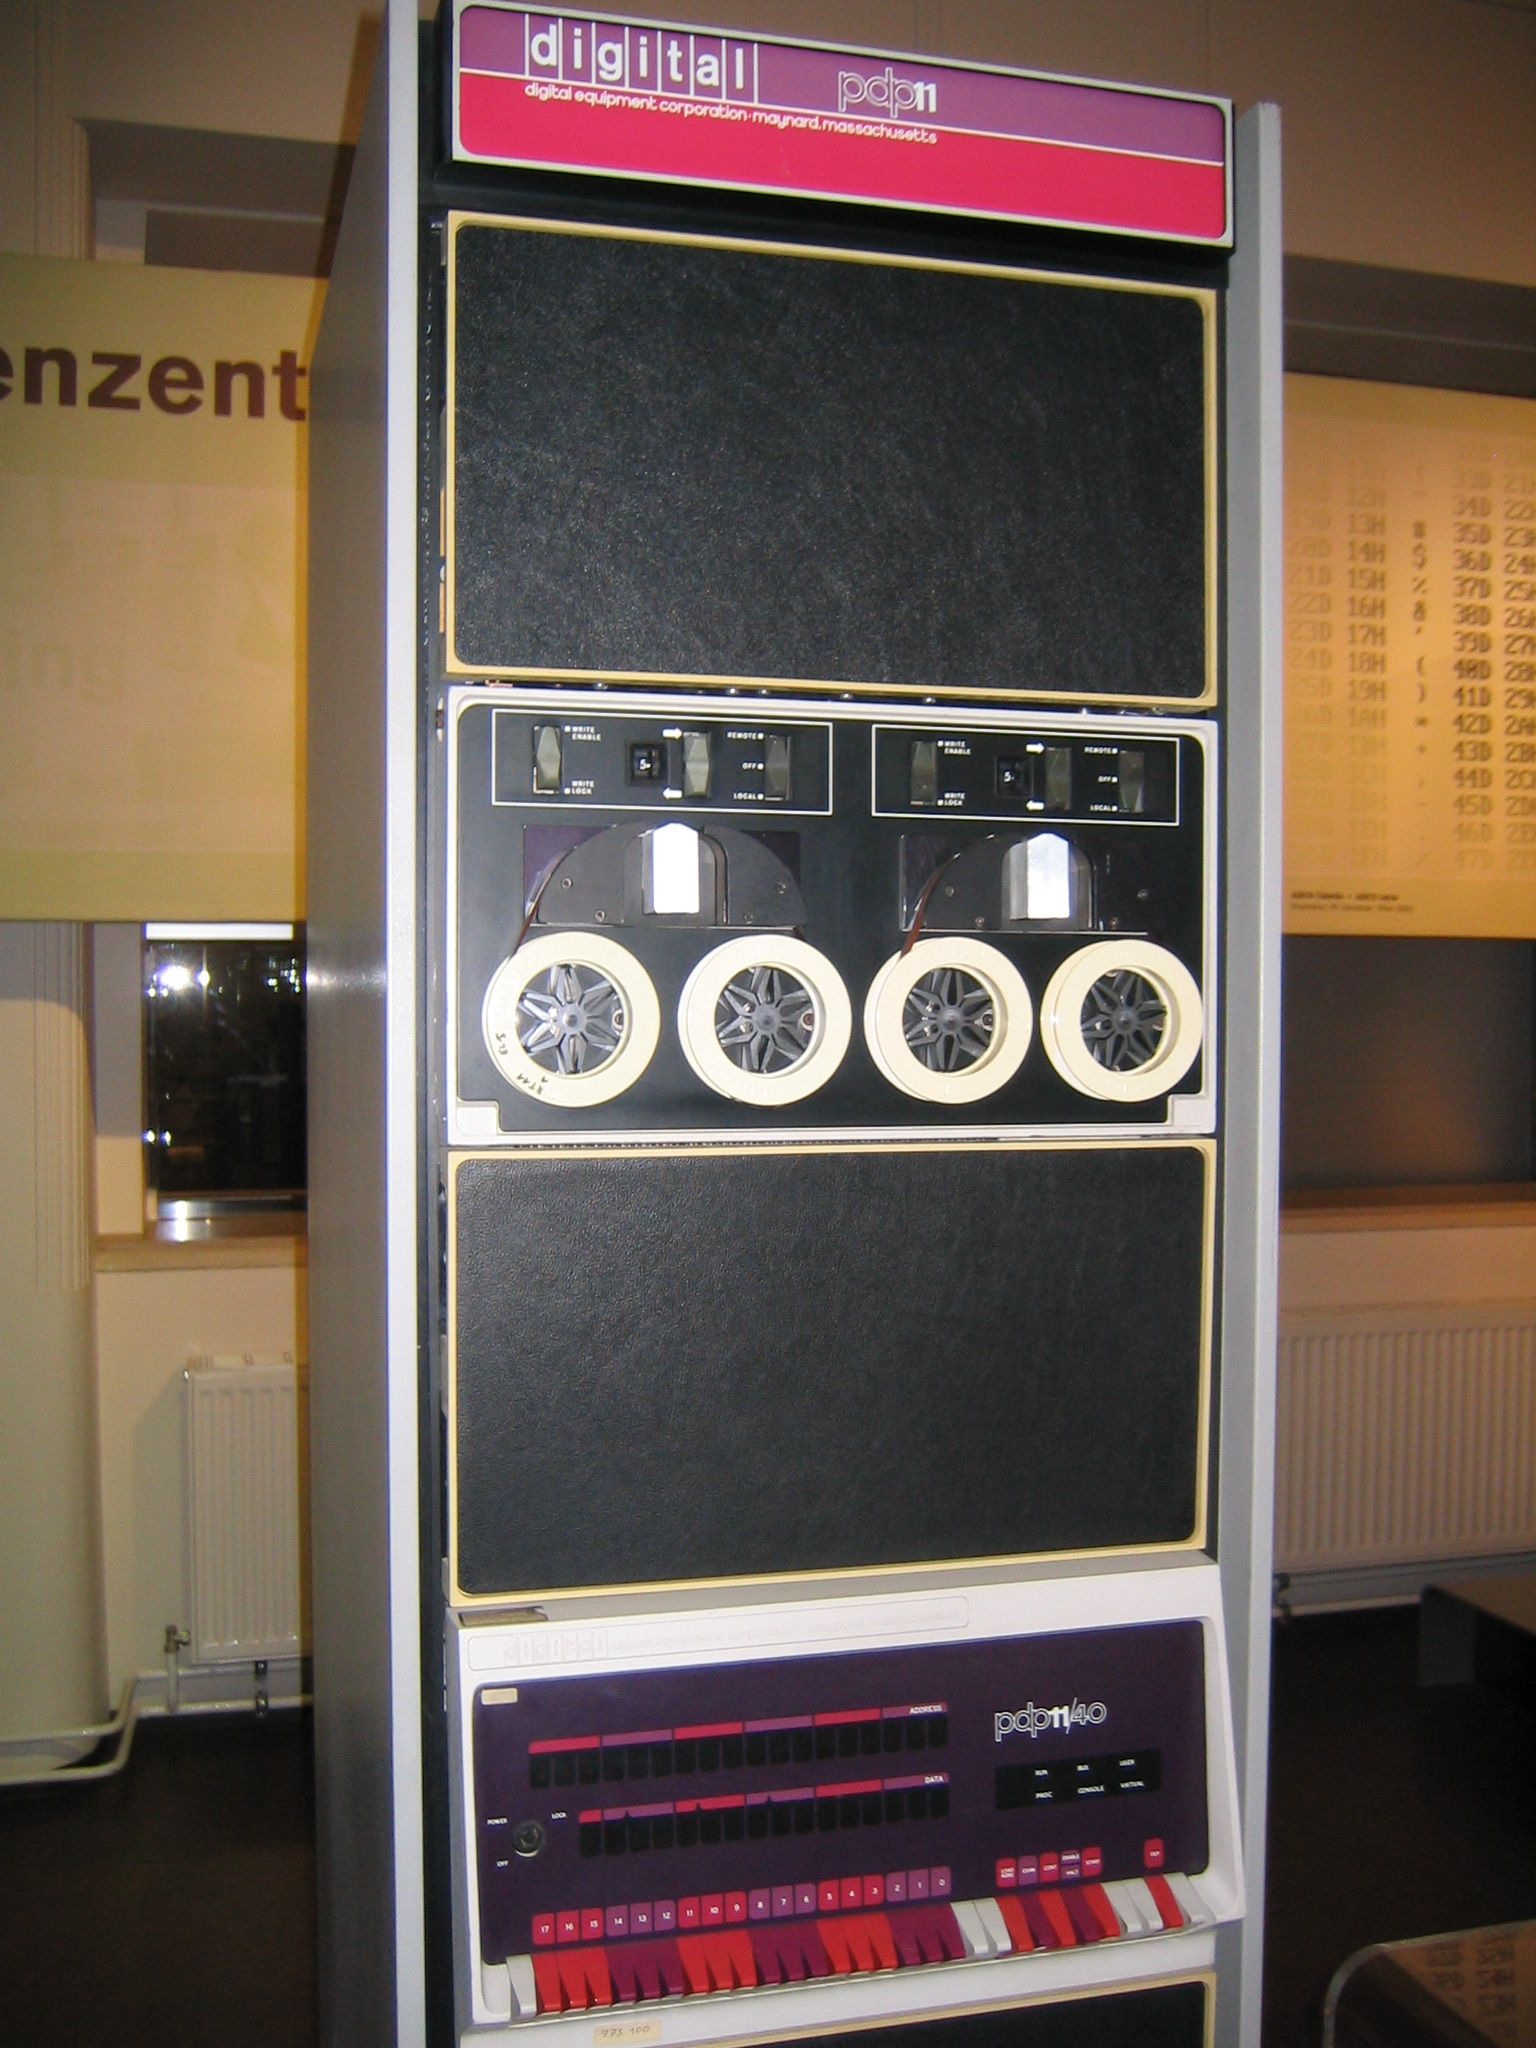
\includegraphics[scale=0.3]
  {./Pictures/Machines-Pictures/PDP-11.jpeg}

  \caption{Komputer PDP-11.}

  \label{fig:PDP-11}

\end{figure}
% ###################





% % ###################
% \begin{figure}

%   \centering


%   \includegraphics[scale=0.3]
%   {./Pictures/Machines-Pictures/PDP-11.jpeg}

%   \caption{Komputer PDP-11.}

%   \label{fig:PDP-11}

% \end{figure}
% % ###################





% ###################
\begin{figure}

  \centering


  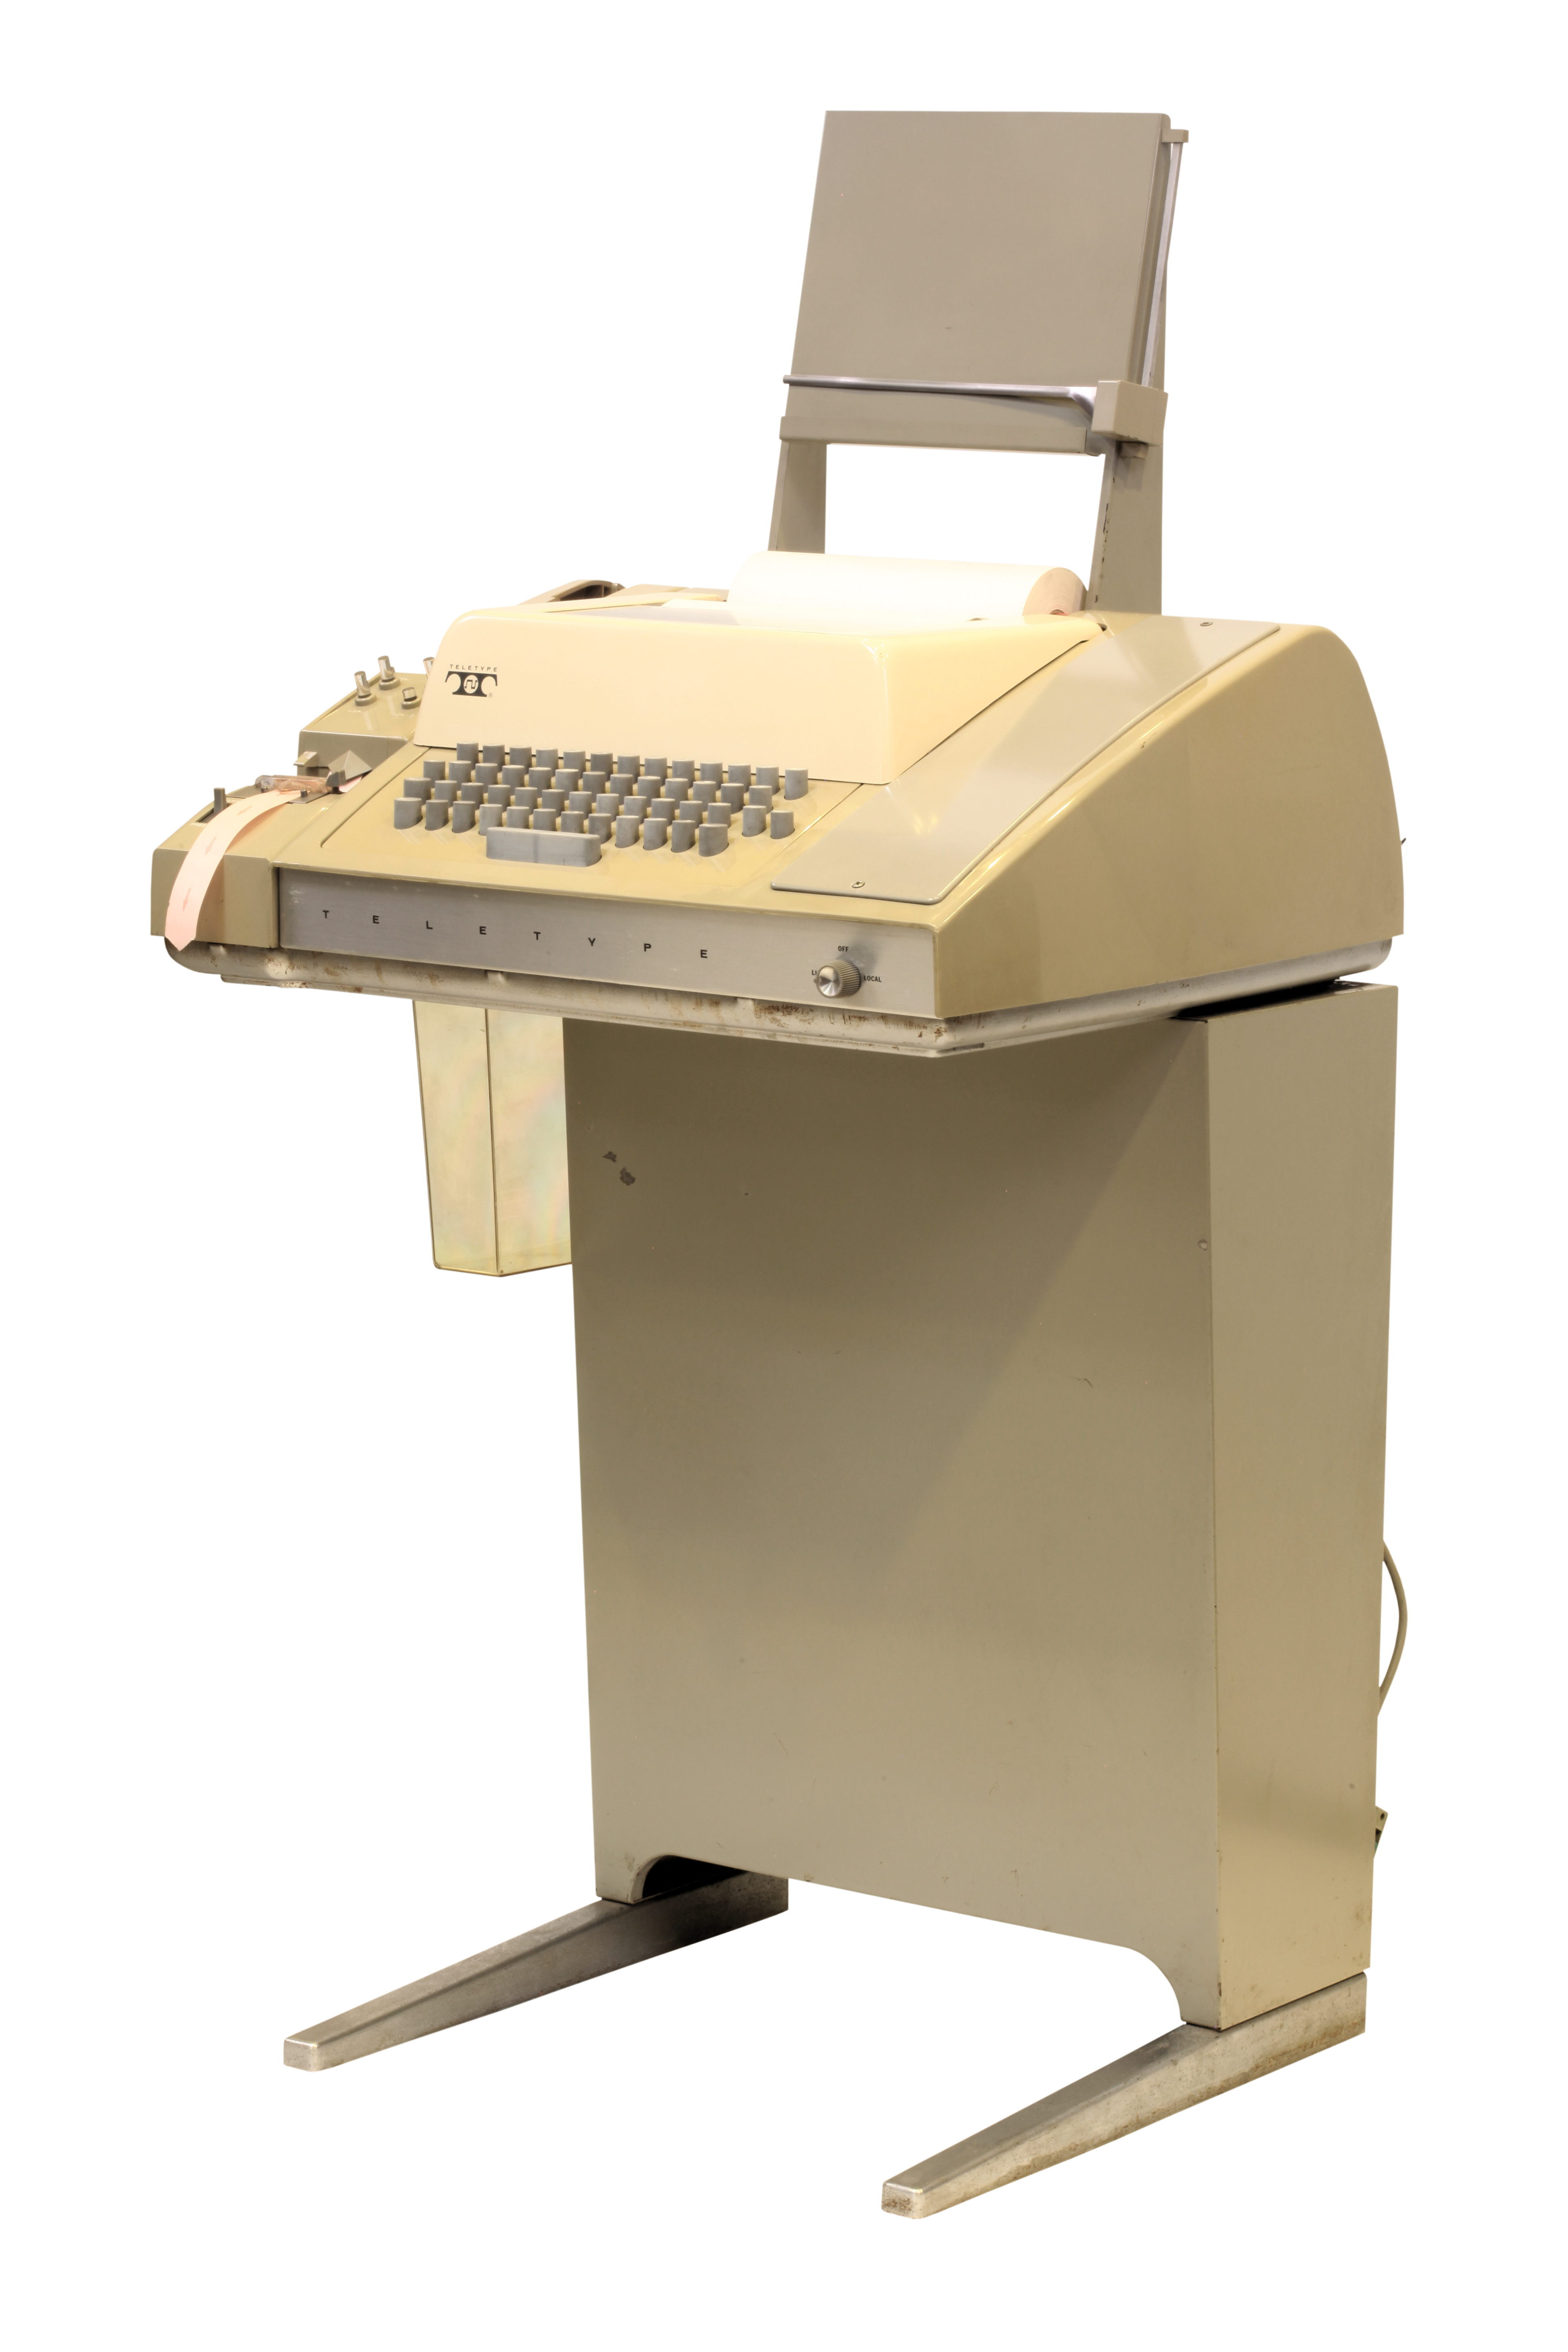
\includegraphics[scale=0.05]
  {./Pictures/Machines-Pictures/Teletype-Model-33-ASR-01.jpeg}
  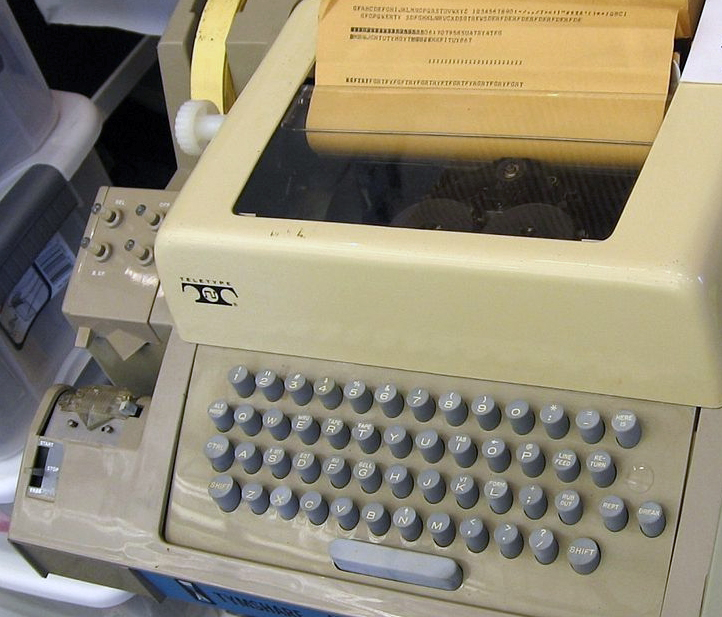
\includegraphics[scale=0.2]
  {./Pictures/Machines-Pictures/Teletype-Model-33-ASR-02.jpeg}

  \caption{Dalekopis Teletype Model~33 firmy Teletype Corporation,
    dostępny w~wersji komercyjnej od 1963~r. Jedna z~pierwszych urządzeń,
    które wspierało system kodowania ASCII. }

  \label{fig:Teletype-Model-33-ASR}

\end{figure}
% ###################





% % ###################
% \begin{figure}

%   \centering


%   \includegraphics[scale=0.5]
%   {./Pictures/Machines-Pictures/Dennis-Ritchie-Ken-Thompson-PDP-11.jpg}

%   \caption{Dennis-Ritchie (stojący) i~Ken Thompson pracują na komputerze
%     \textsc{pdp}-11.}

%   \label{fig:Ritchie-Thompson-PDP-11}

% \end{figure}
% % ###################
























% ####################################################################
% ####################################################################
% Bibliography

\printbibliography





% ############################

% End of the document
\end{document}
